% no chapters, left justify equations
\documentclass[a4paper,11pt,fleqn,oneside]{book}

% input encoding
\usepackage[utf8]{inputenc}
\usepackage[OT1]{fontenc}

% better hyphenation

\usepackage[english]{babel}
\usepackage{color}
\definecolor{grau}{rgb}{0.3, 0.3, 0.3}
% used packages
\usepackage{amssymb,amsmath}
\usepackage{epsfig,graphicx}
\usepackage{xifthen}
\usepackage{multirow}
\usepackage{rotating}
\usepackage{enumitem}


\usepackage{hyperref}
\setcounter{tocdepth}{3}
\setlength{\parindent}{0in}


\begin{document}
\tableofcontents


\chapter{Documentation}

\begin{itemize}

\item[10.02.2012]
wrote E-Mail to Andrew about performance problems and wavelenght computation error 
in \texttt{fuenfincr256\_1} \\
started some runs with higher central delta and broader smoothing lenghts, i.e. 
32/dx and 100/dx; all 128 resolution except second last one (same seed!): 
\begin{verbatim}
83492 0.60500 d31c_1_sta harre   r     02/10/2012 15:19:56 intel.q@astro18  16        
83493 0.60500 d31c_2_sta harre   r     02/10/2012 15:20:37 intel.q@astro29  16        
83494 0.60500 d31c_3_sta harre   r     02/10/2012 15:21:17 intel.q@astro25  16        
83495 0.60500 d51c_sl100 harre   r     02/10/2012 15:23:21 intel.q@astro31  16  
83496 0.54786 d3+3c_sl50 harre   r     02/10/2012 15:37:13 intel.q@astro12  16        
83497 0.60500 d3+3c_sl50 harre   r     02/10/2012 15:39:16 intel.q@astro30  32  
83498 0.60500 d15+3c_sl5 harre   r     02/10/2012 15:44:23 intel.q@astro30  16        
\end{verbatim}

\item[09.02.2012]
\texttt{drd5\_r256} last written to hdf5 file feb 09, 05:07 \\
\texttt{fuenfincr256\_2} last written to hdf5 file feb 06, 03:28 \\
\texttt{drd5\_r256\_2} last written to hdf5 file feb 07, 00:50 \\

\item[02.02.2012]
\texttt{drdx\_h100\_128\_1} run has again severe consistency 
metric problem \\ $\rightarrow$ not clear why \\
upper python script does not work, was commented out again \\
plan: \textbf{move to python scripts in general in order to have
 easier arithmetic calculations} \\   
plan: create new folder structure and remove old simulations $\rightarrow$ done \\

\item[31.01.2012]
note: h=70.3 in galacticus xml input file is expected, consistent tree obviously implies it \\
$\rightarrow$ fixed: changed in markus parameter file for the converter and in xml file \\
$\rightarrow$ question: why not read out? \\
$\rightarrow$ python updateGalacticusStart.py from Markus 

\item[30.01.2012]
new consistenttree with vmax=20



\end{itemize}

\chapter{Simulations} %%%%%%%%%%%%%%%%%%%%%%%%%%%%%%%%%%%%%%%%%%%%%%%%%%%%%%%%%%%%%%%

\section{r128} %%%%%%%%%%%%%%%%%%%%%%%%%%%%%%%%%%%%%%%%%%%%%%%%%%%%%%%%%%%%%%%%%%%%%%

\subsection{h70} %%%%%%%%%%%%%%%%%%%%%%%%%%%%%%%%%%%%%%%%%%%%%%%%%%%%%%%%%%%%%%%%%%%%

\newpage
\subsection{h100} %%%%%%%%%%%%%%%%%%%%%%%%%%%%%%%%%%%%%%%%%%%%%%%%%%%%%%%%%%%%%%%%%%%

\subsubsection{drdx\_3} 

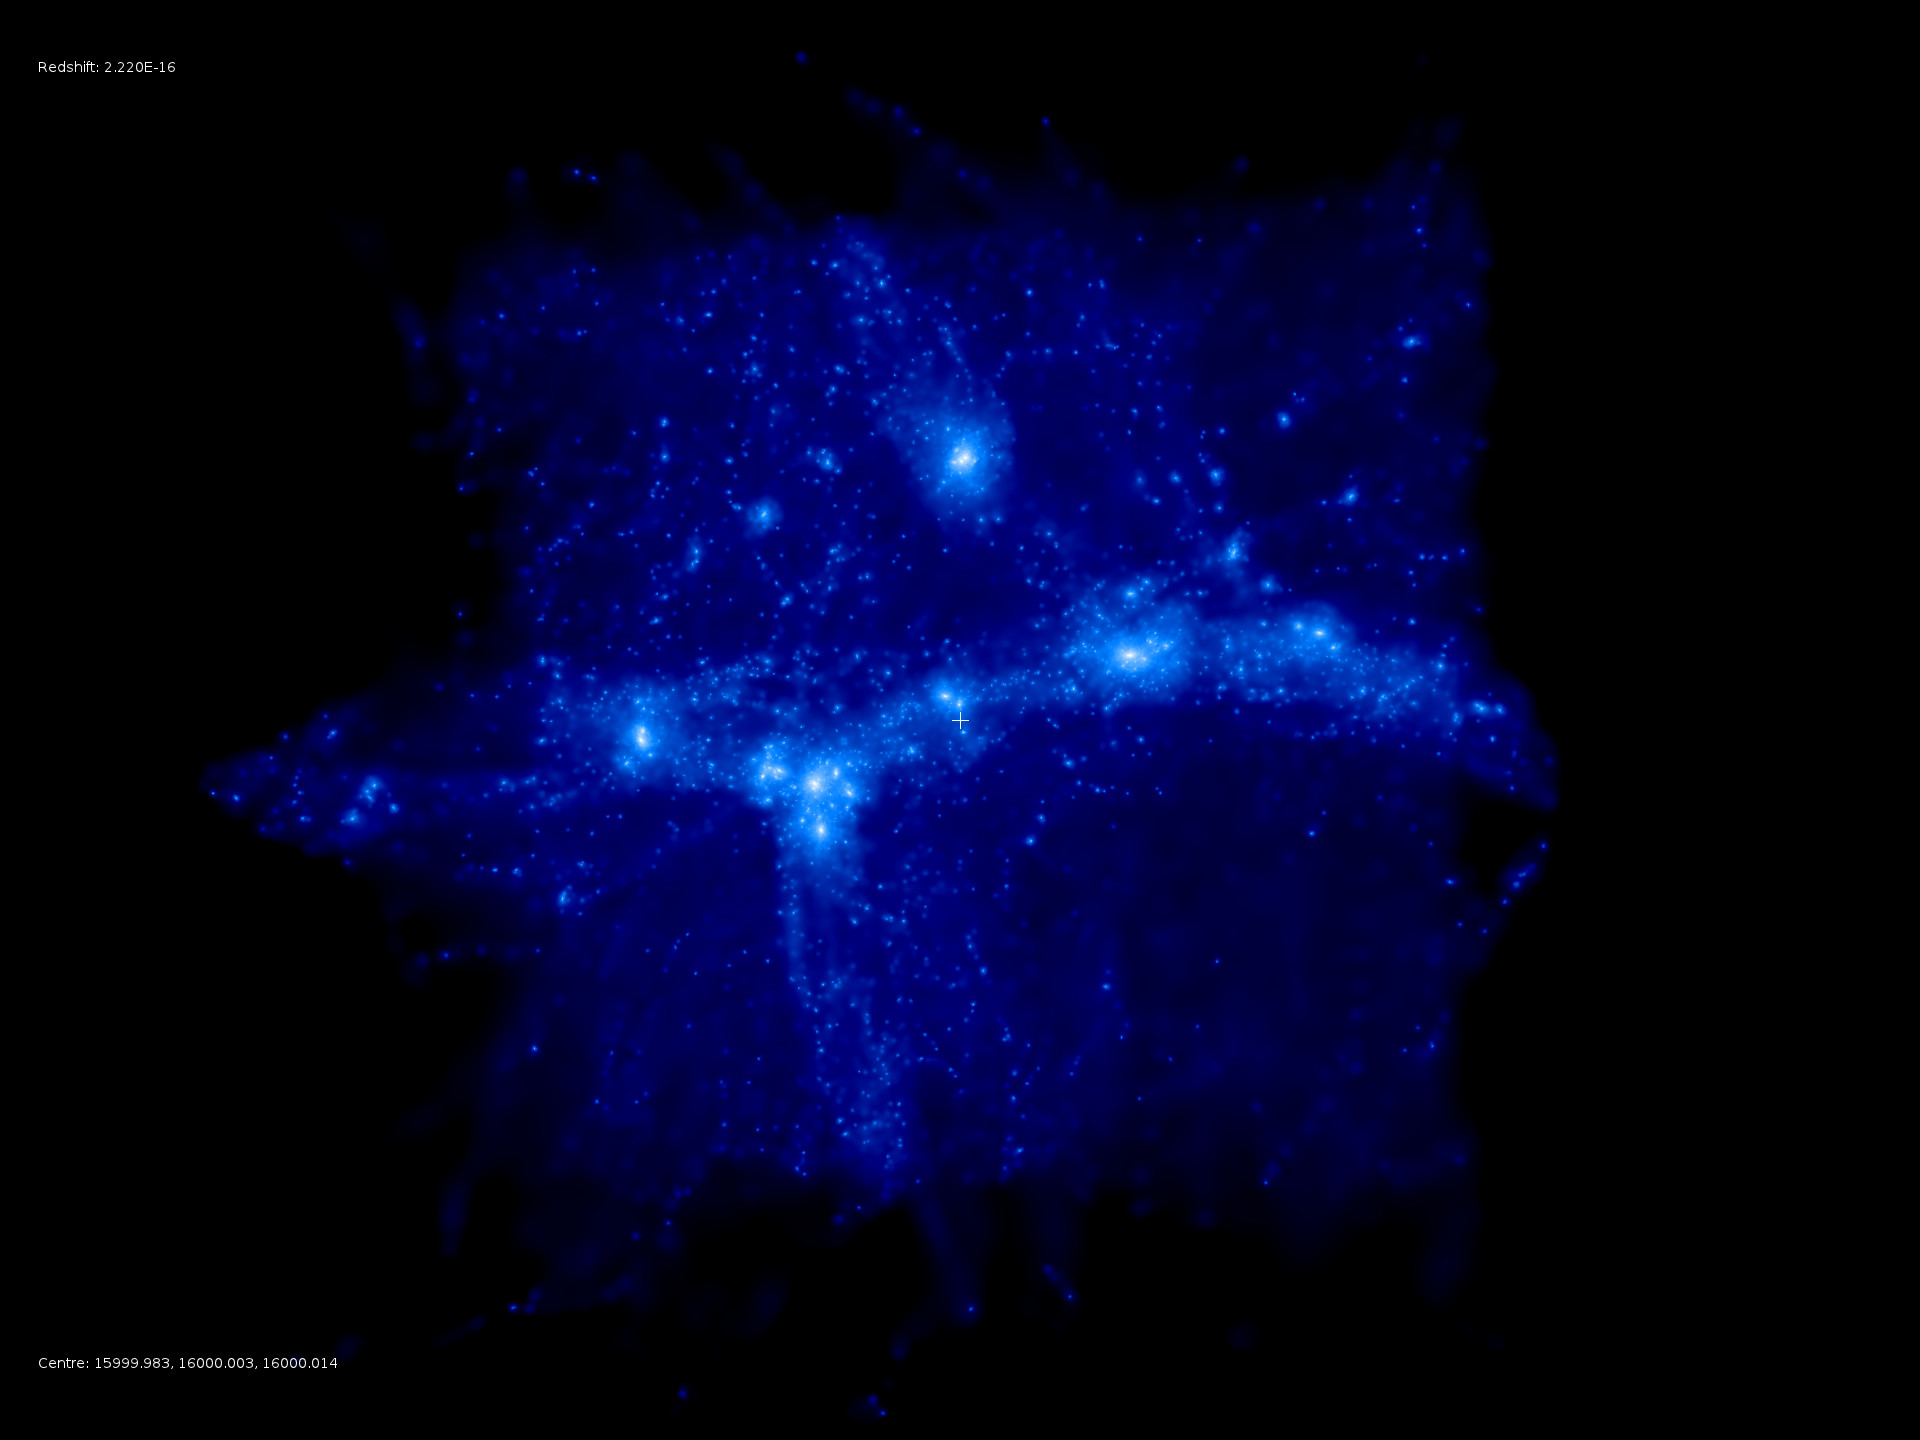
\includegraphics[scale=0.12]{drdx_3/rotate_00185.jpg} 
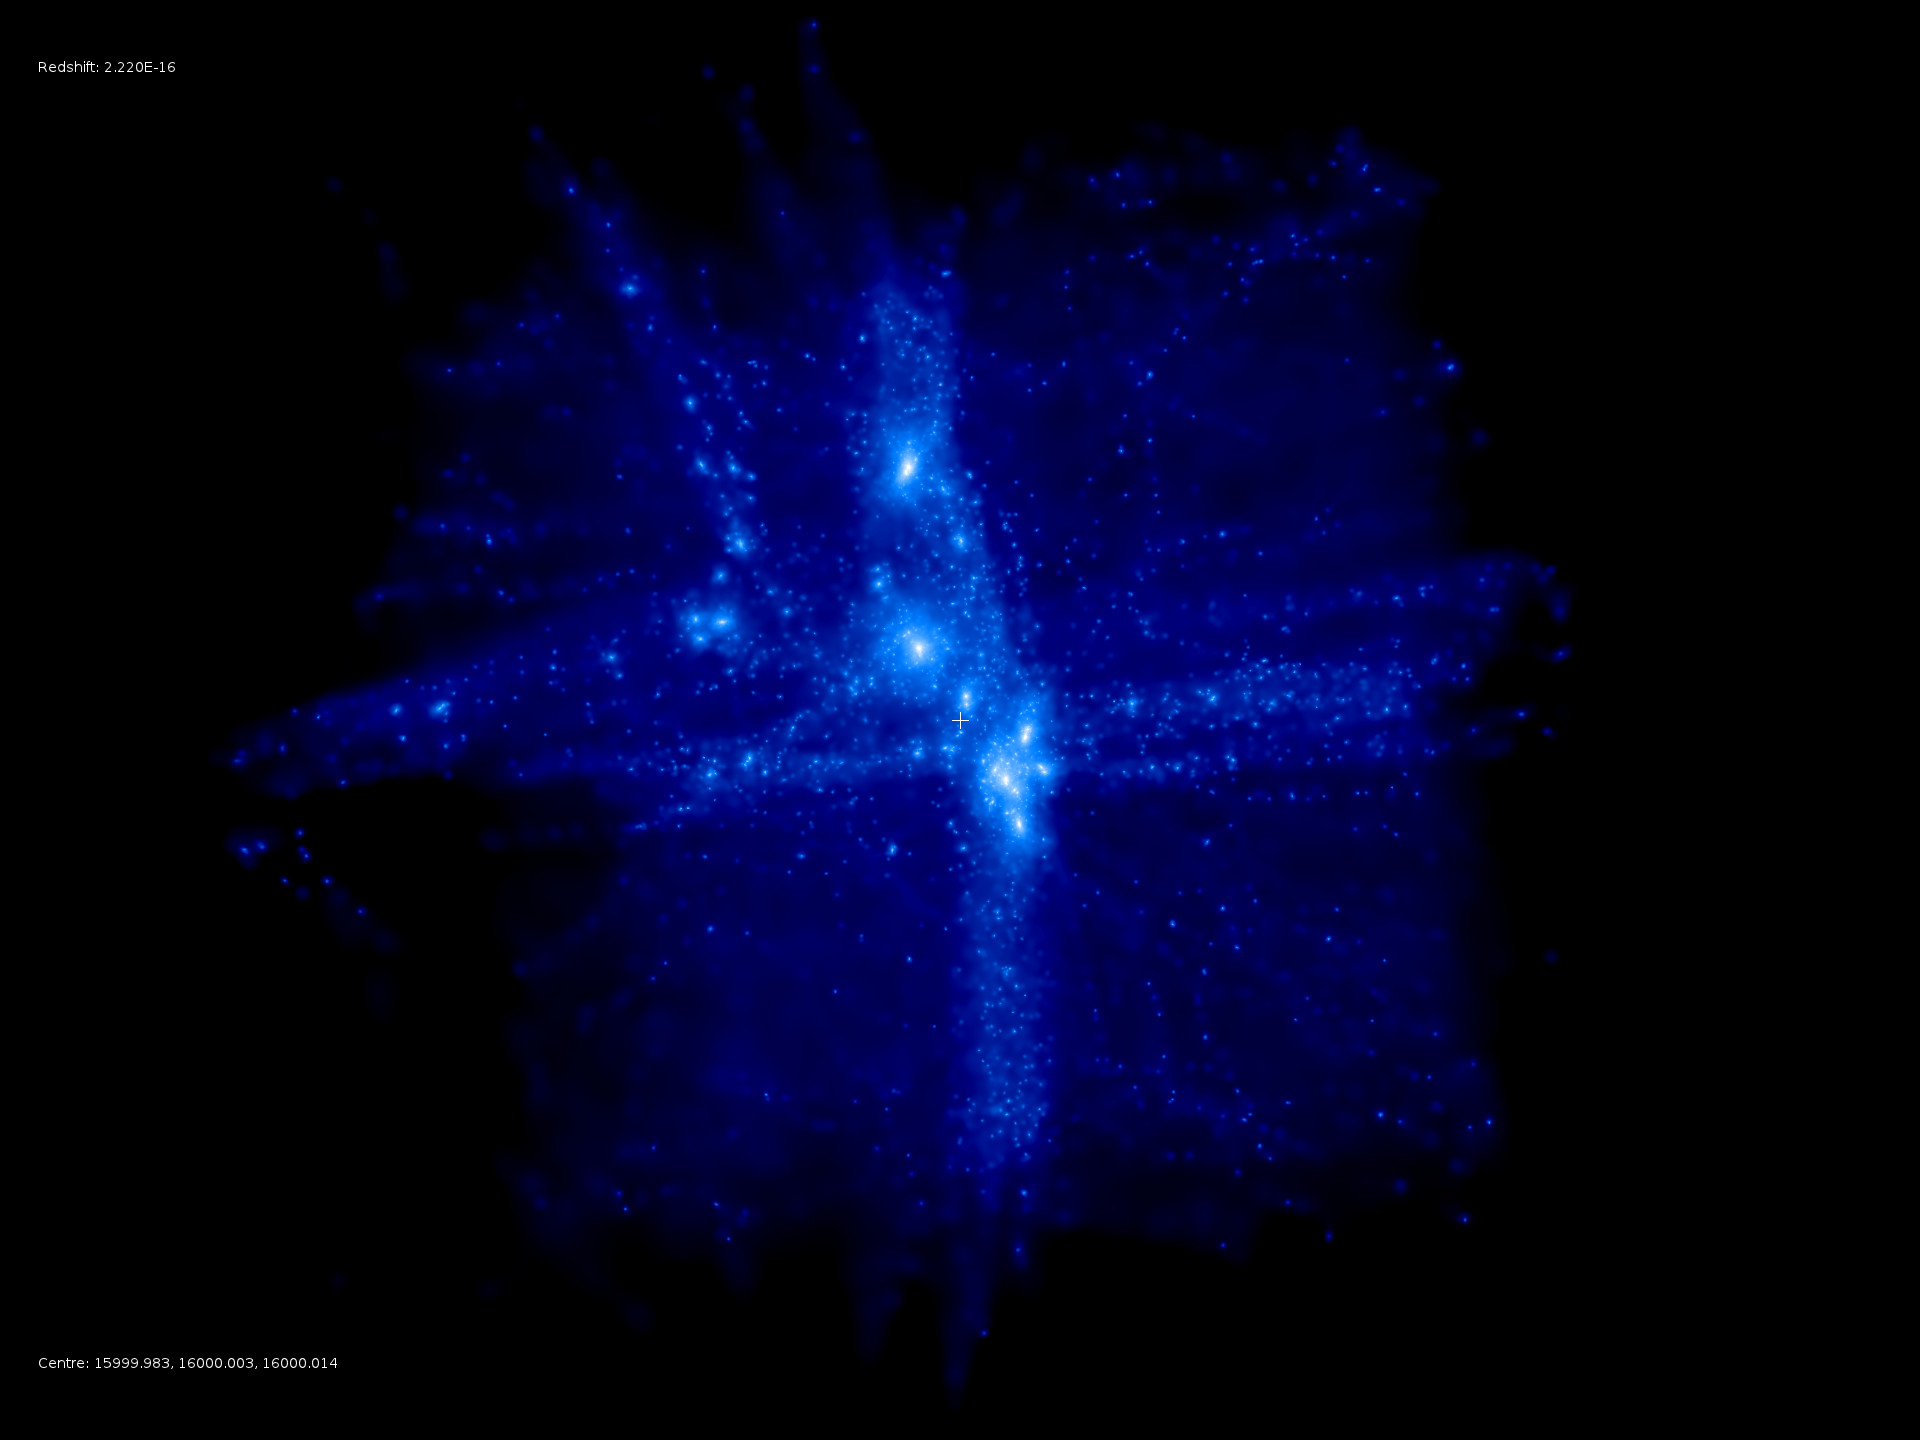
\includegraphics[scale=0.12]{drdx_3/rotate_00136.jpg} 

\textsc{rockstarred} $\surd$  \\
pfff $\rightarrow$ Error: too few halos at scale factor 0.926072 to calculate consistency metric.

\newpage
\subsubsection{drdx\_h100\_r128\_1}

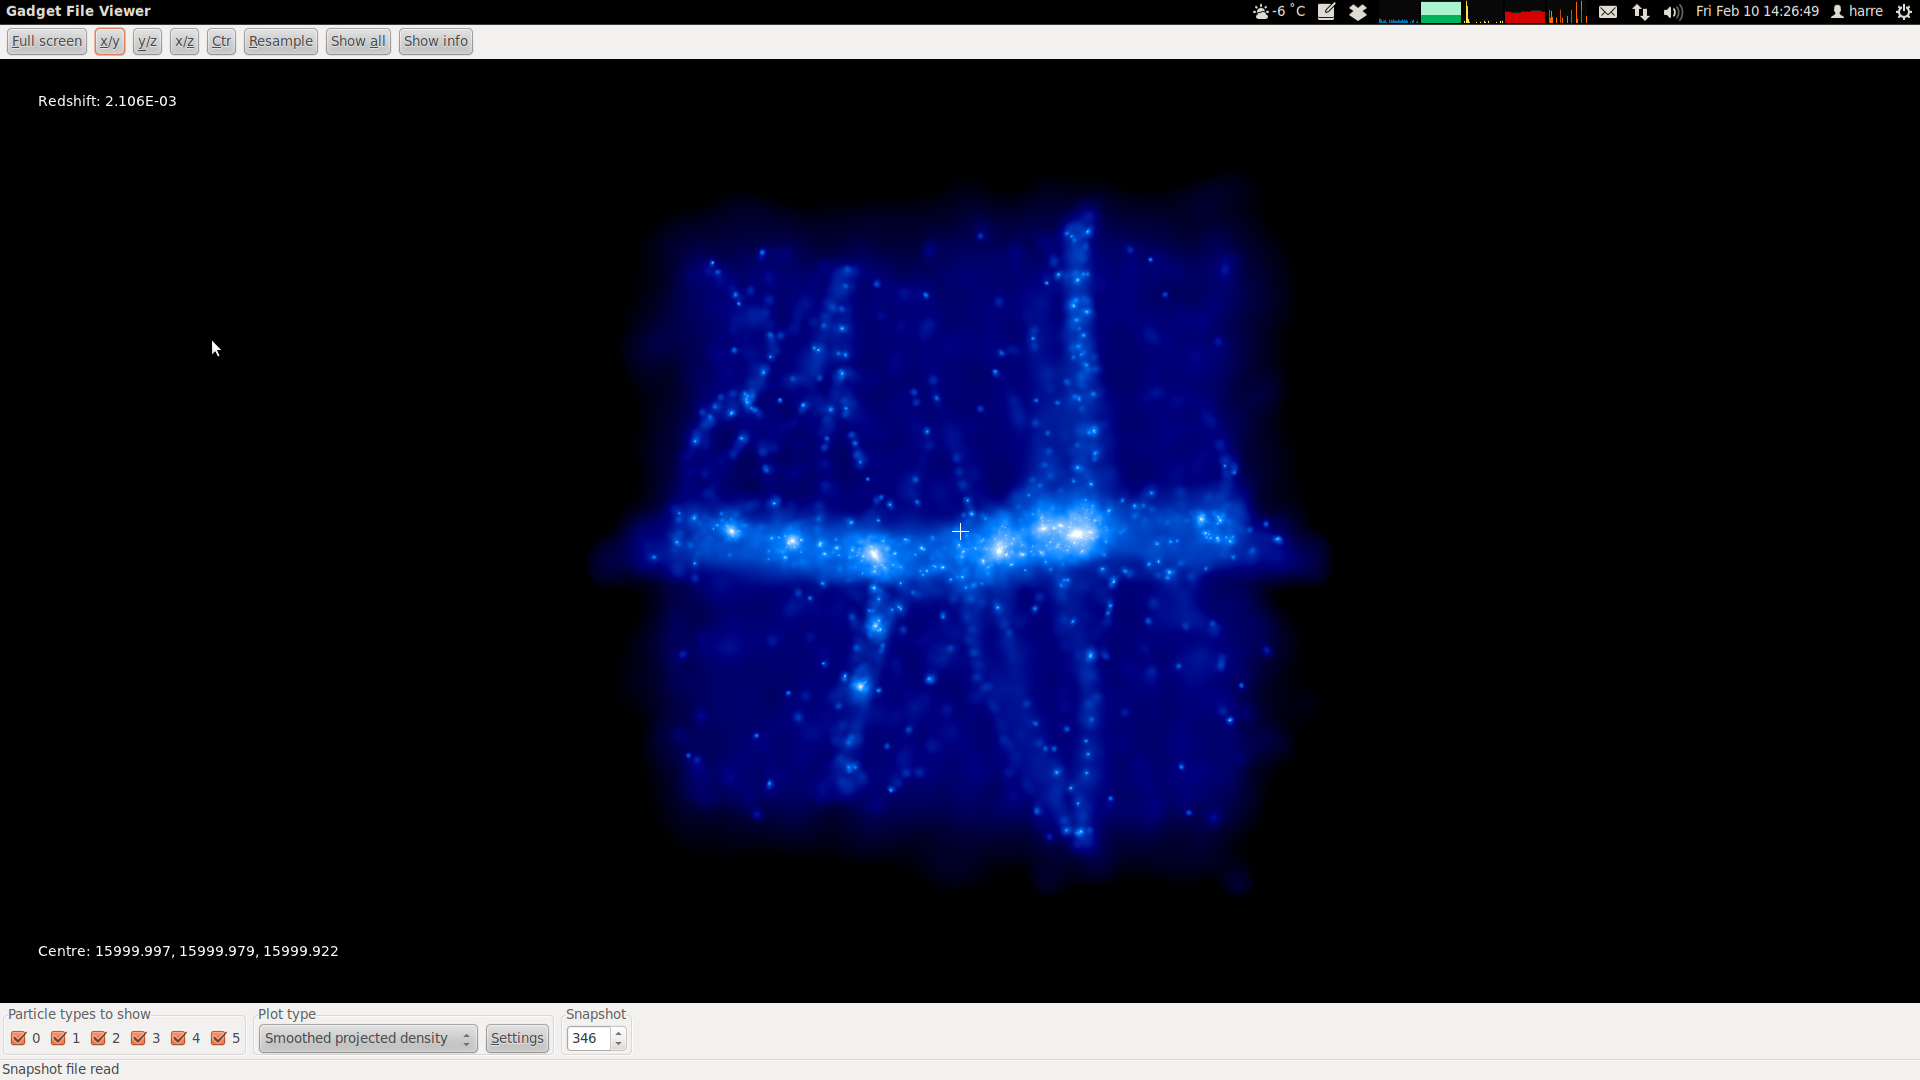
\includegraphics[scale=0.12]{drdx_h100_r128_1/1.png} 
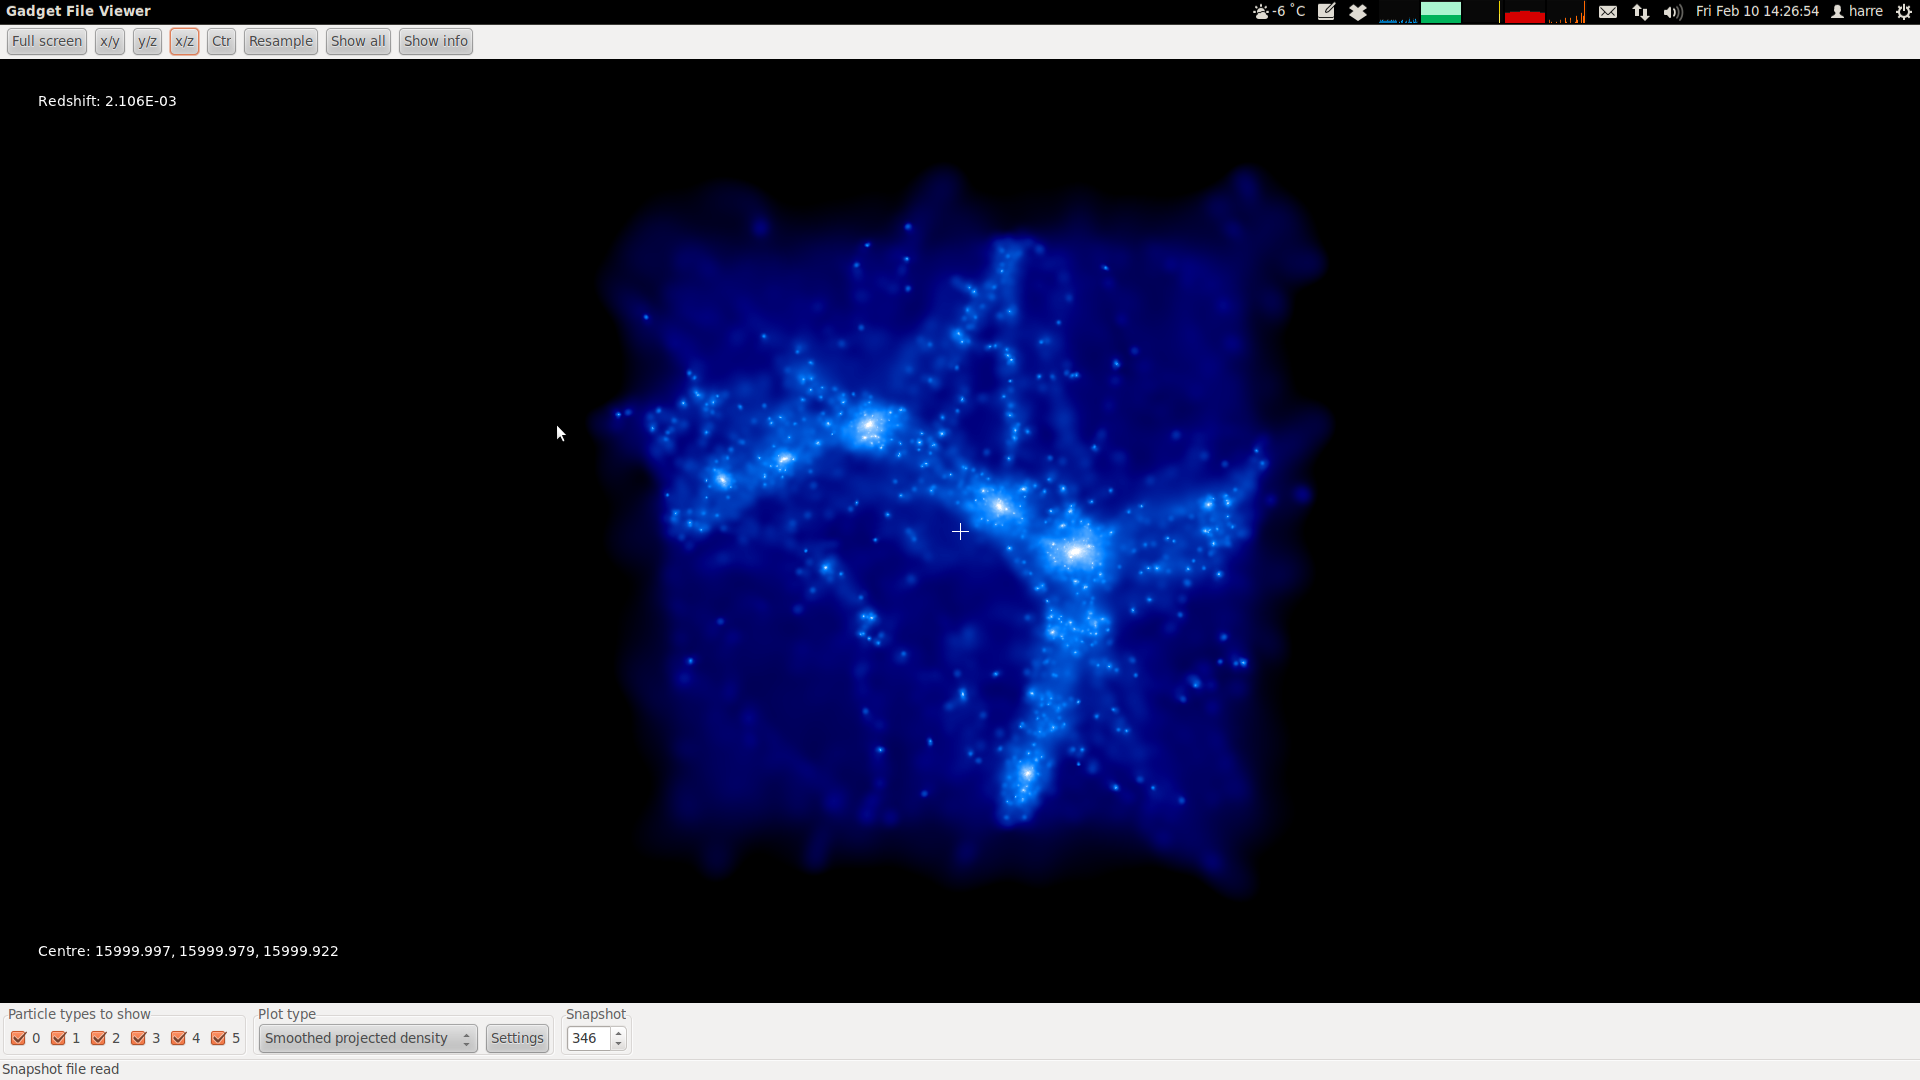
\includegraphics[scale=0.12]{drdx_h100_r128_1/2.png} 

\textsc{rockstarred} $\surd$  \\
consistenttree: too few halos at scale factor 0.896 ... $\rightarrow$ wtf? 

\newpage
\subsubsection{drdx\_h100\_r128\_2}

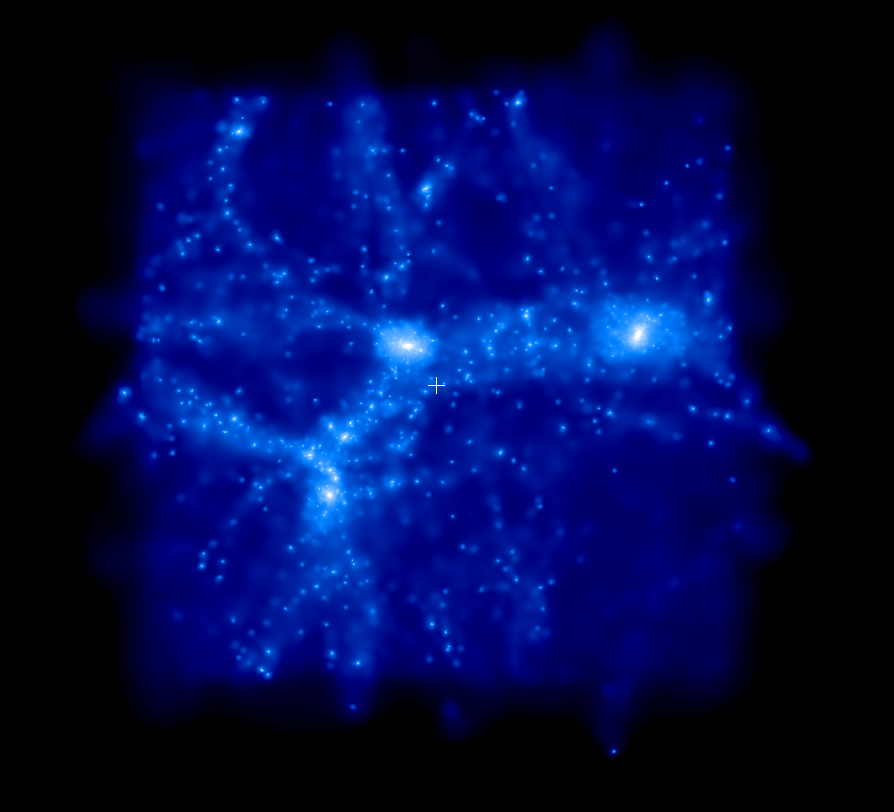
\includegraphics[scale=0.12]{drdx_h100_r128_2/1.png} 
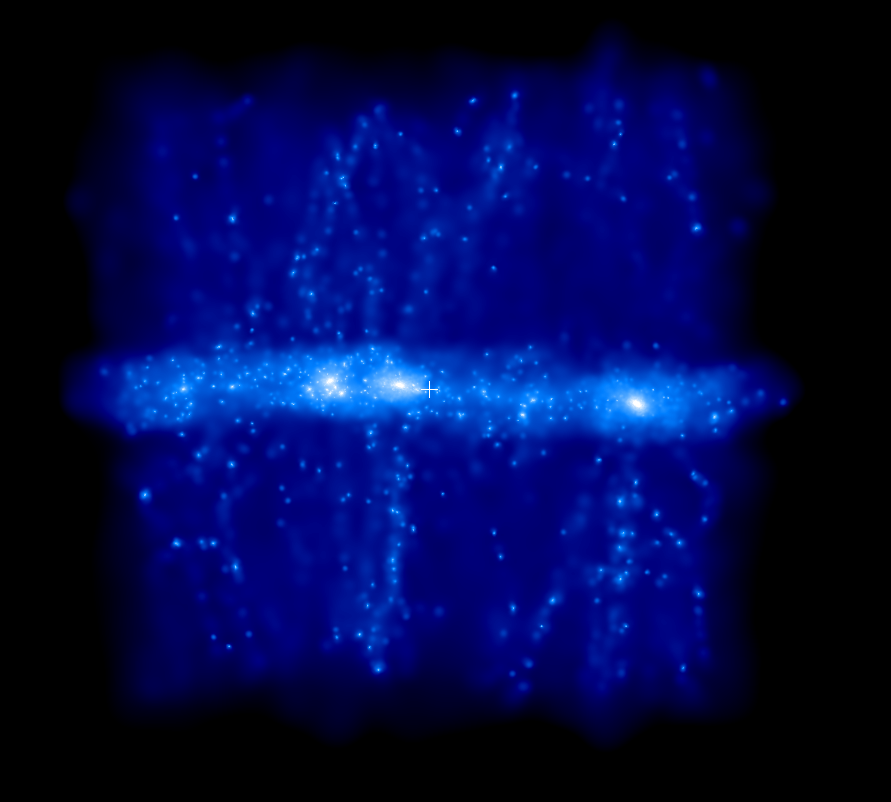
\includegraphics[scale=0.12]{drdx_h100_r128_2/2.png} 
is being rockstarred 




\newpage
\section{r256} %%%%%%%%%%%%%%%%%%%%%%%%%%%%%%%%%%%%%%%%%%%%%%%%%%%%%%%%%%%%%%%%%%%%%%

\newpage
\subsection{h70} %%%%%%%%%%%%%%%%%%%%%%%%%%%%%%%%%%%%%%%%%%%%%%%%%%%%%%%%%%%%%%%%%%%%
 
\newpage
\subsection{h100} %%%%%%%%%%%%%%%%%%%%%%%%%%%%%%%%%%%%%%%%%%%%%%%%%%%%%%%%%%%%%%%%%%%

\subsubsection{drd5\_r256} 

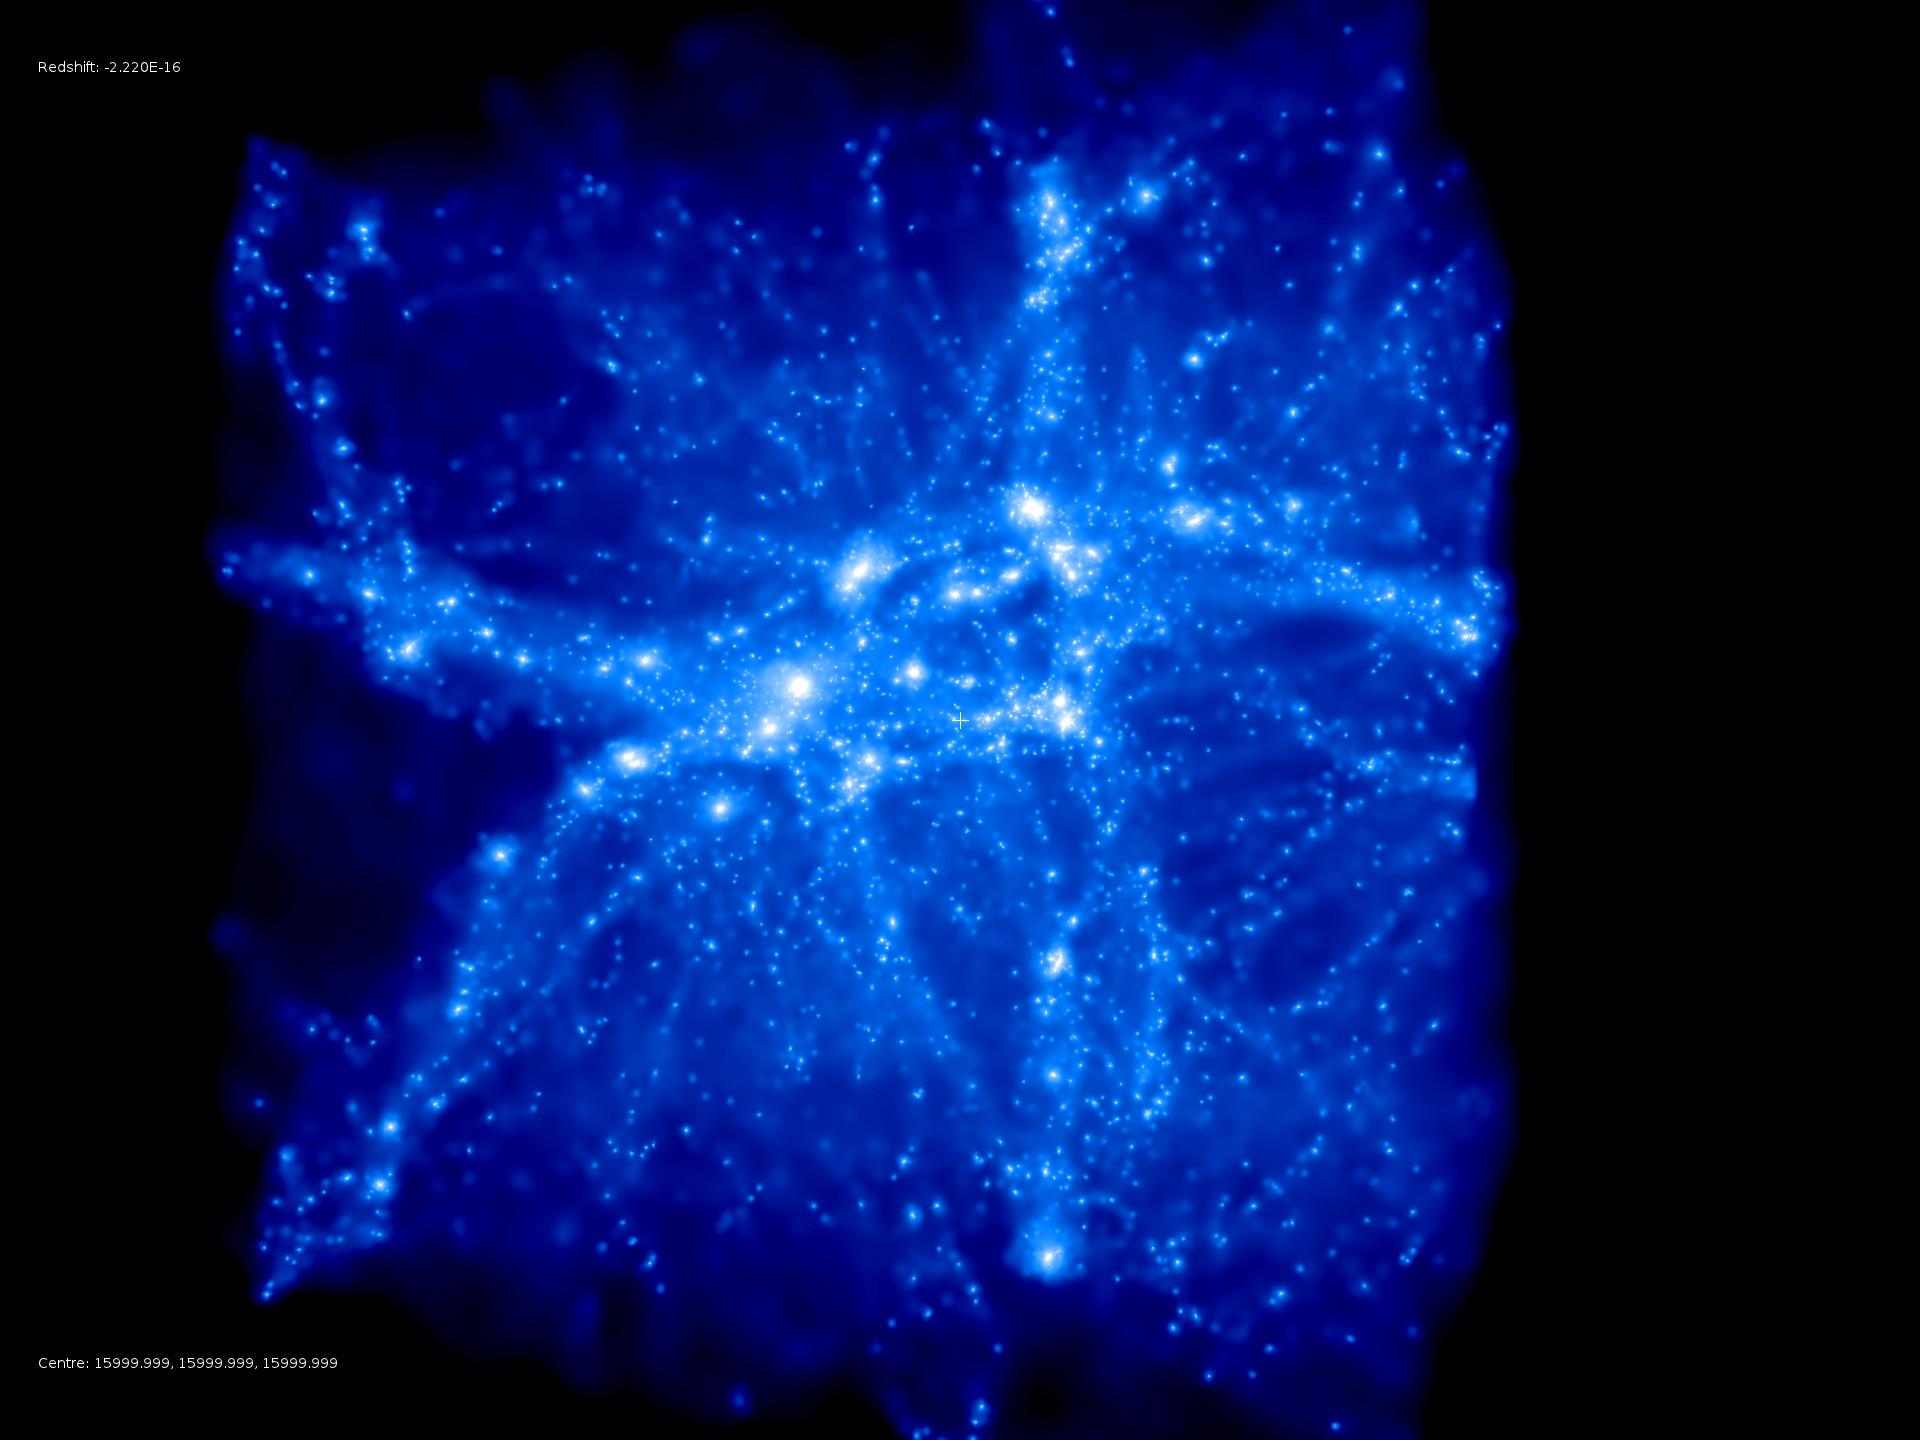
\includegraphics[scale=0.12]{drd5_r256/rotate_00185.jpg} 
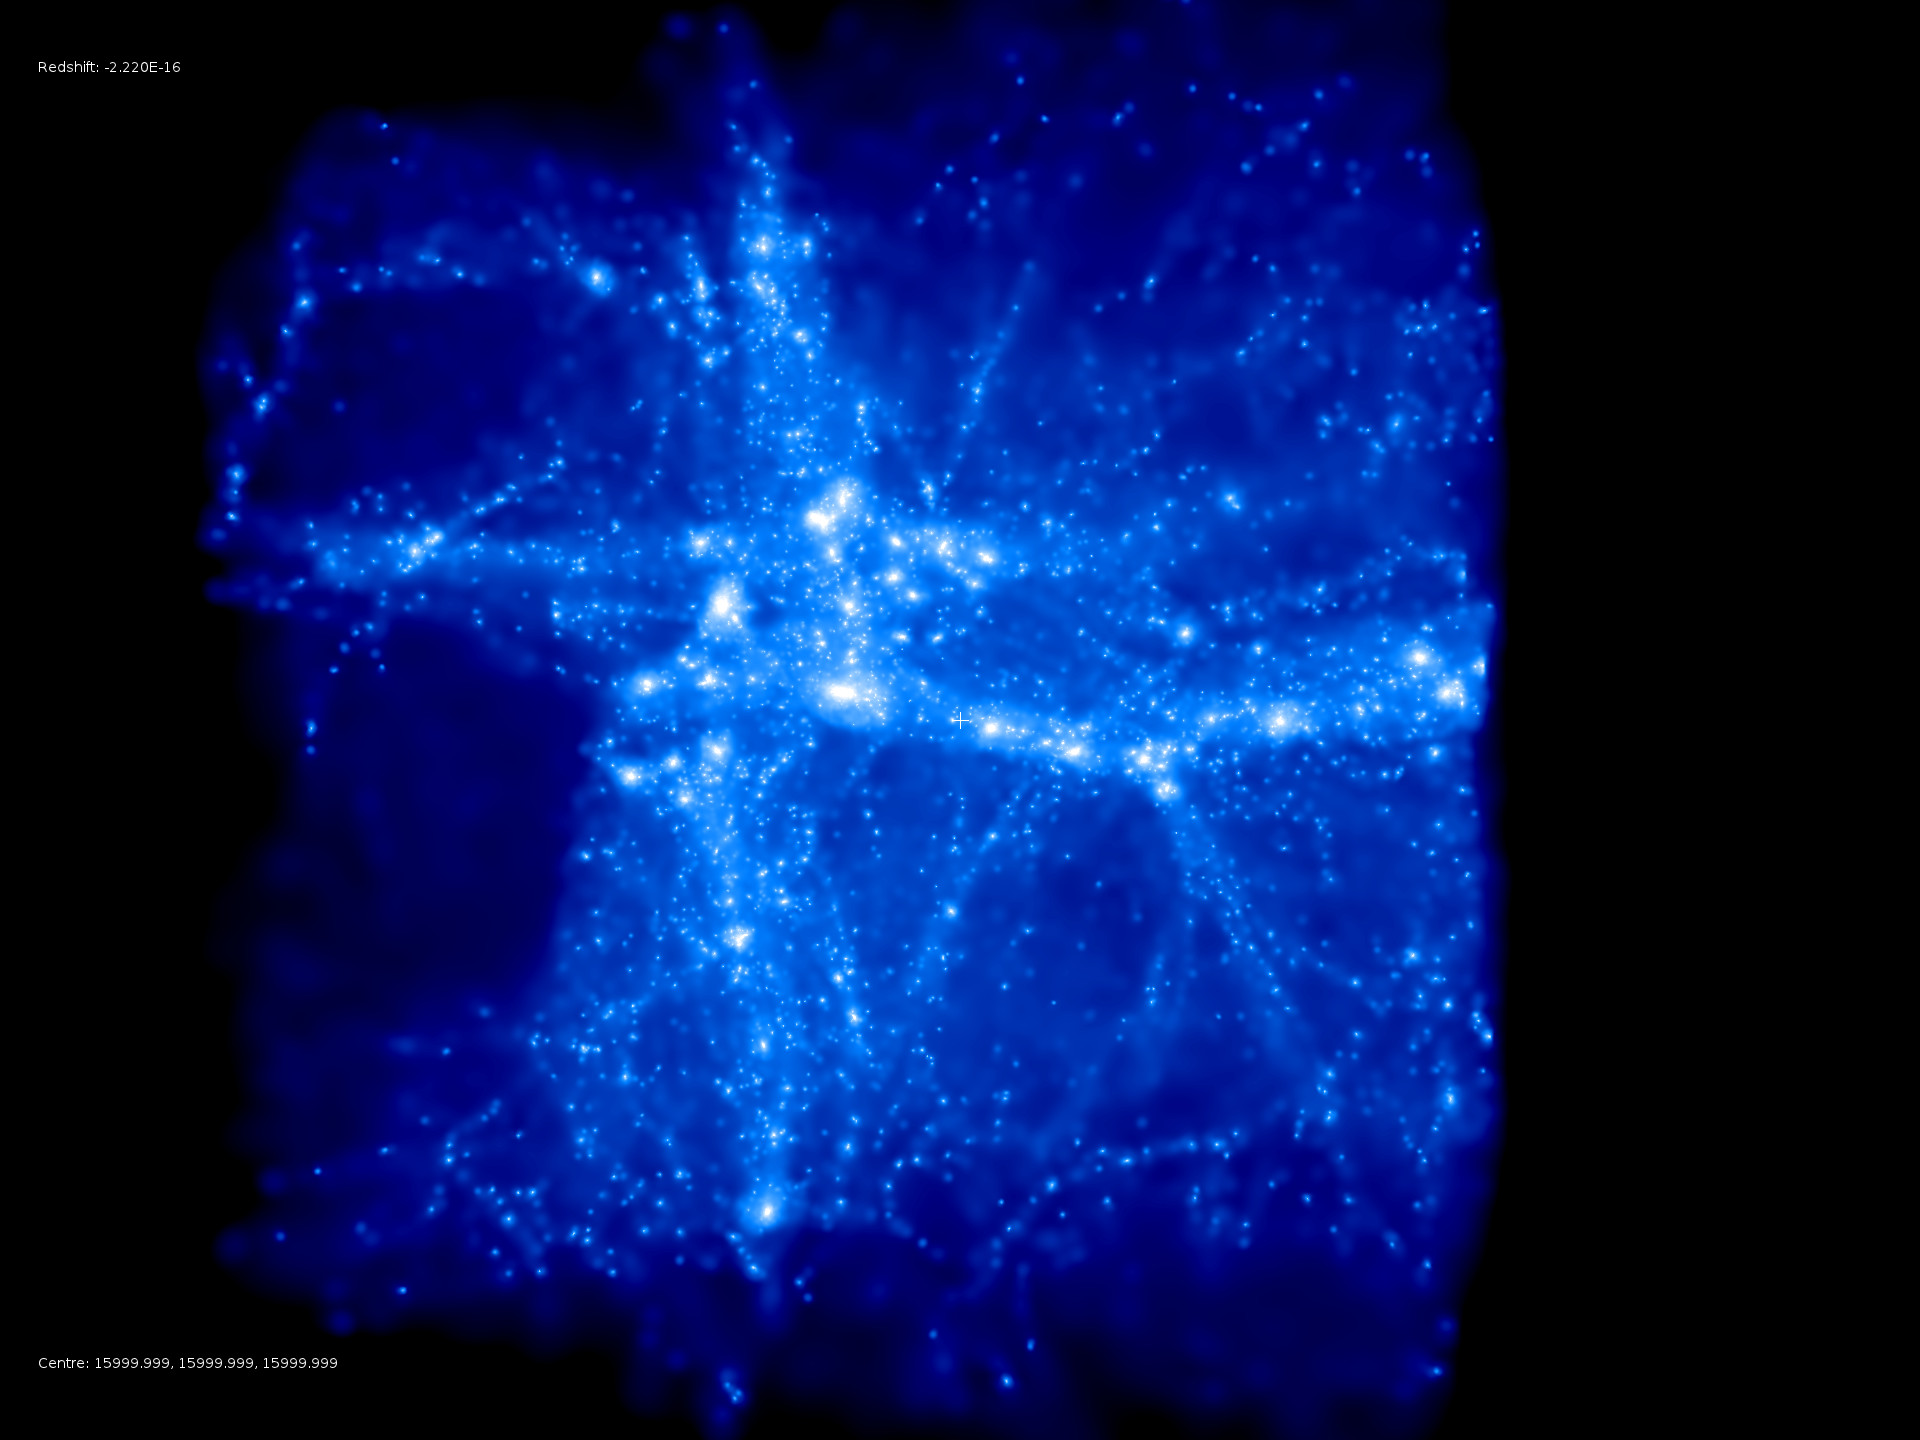
\includegraphics[scale=0.12]{drd5_r256/rotate_00136.jpg} 

\textsc{rockstarred} $\surd$ \\ \textsc{consistenttreed} $\surd$  \\ \textsc{galacticus}: 
\begin{verbatim}
Fatal error in Build_Descendent\_Pointers():
failed to find descendent node: 5546454 of 5522259
galacticus.sh: line 67: 25689 Aborted  
\end{verbatim}
tree copied to markus transfer \\
$\rightarrow$ re-converted with bugfixed converter \\
galacticus running on SGE

\newpage
\subsubsection{drd5\_r256\_2 $\rightarrow$ dump!} 

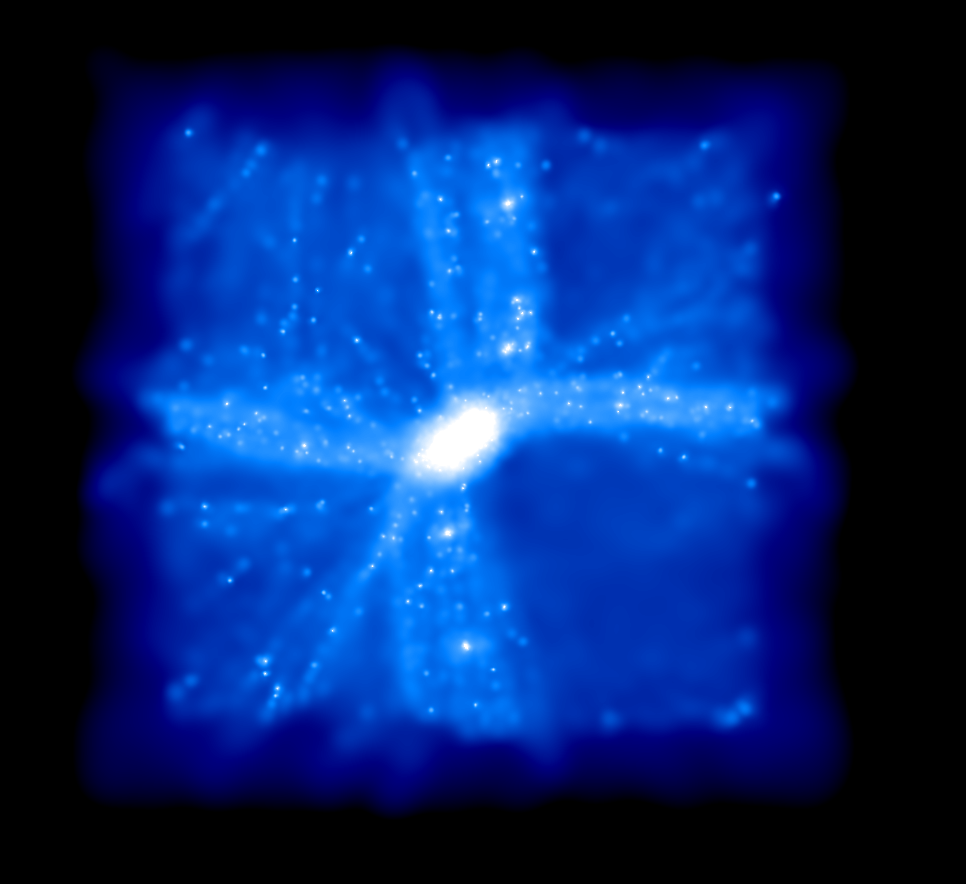
\includegraphics[scale=0.12]{drd5_r256_2/1.png} 
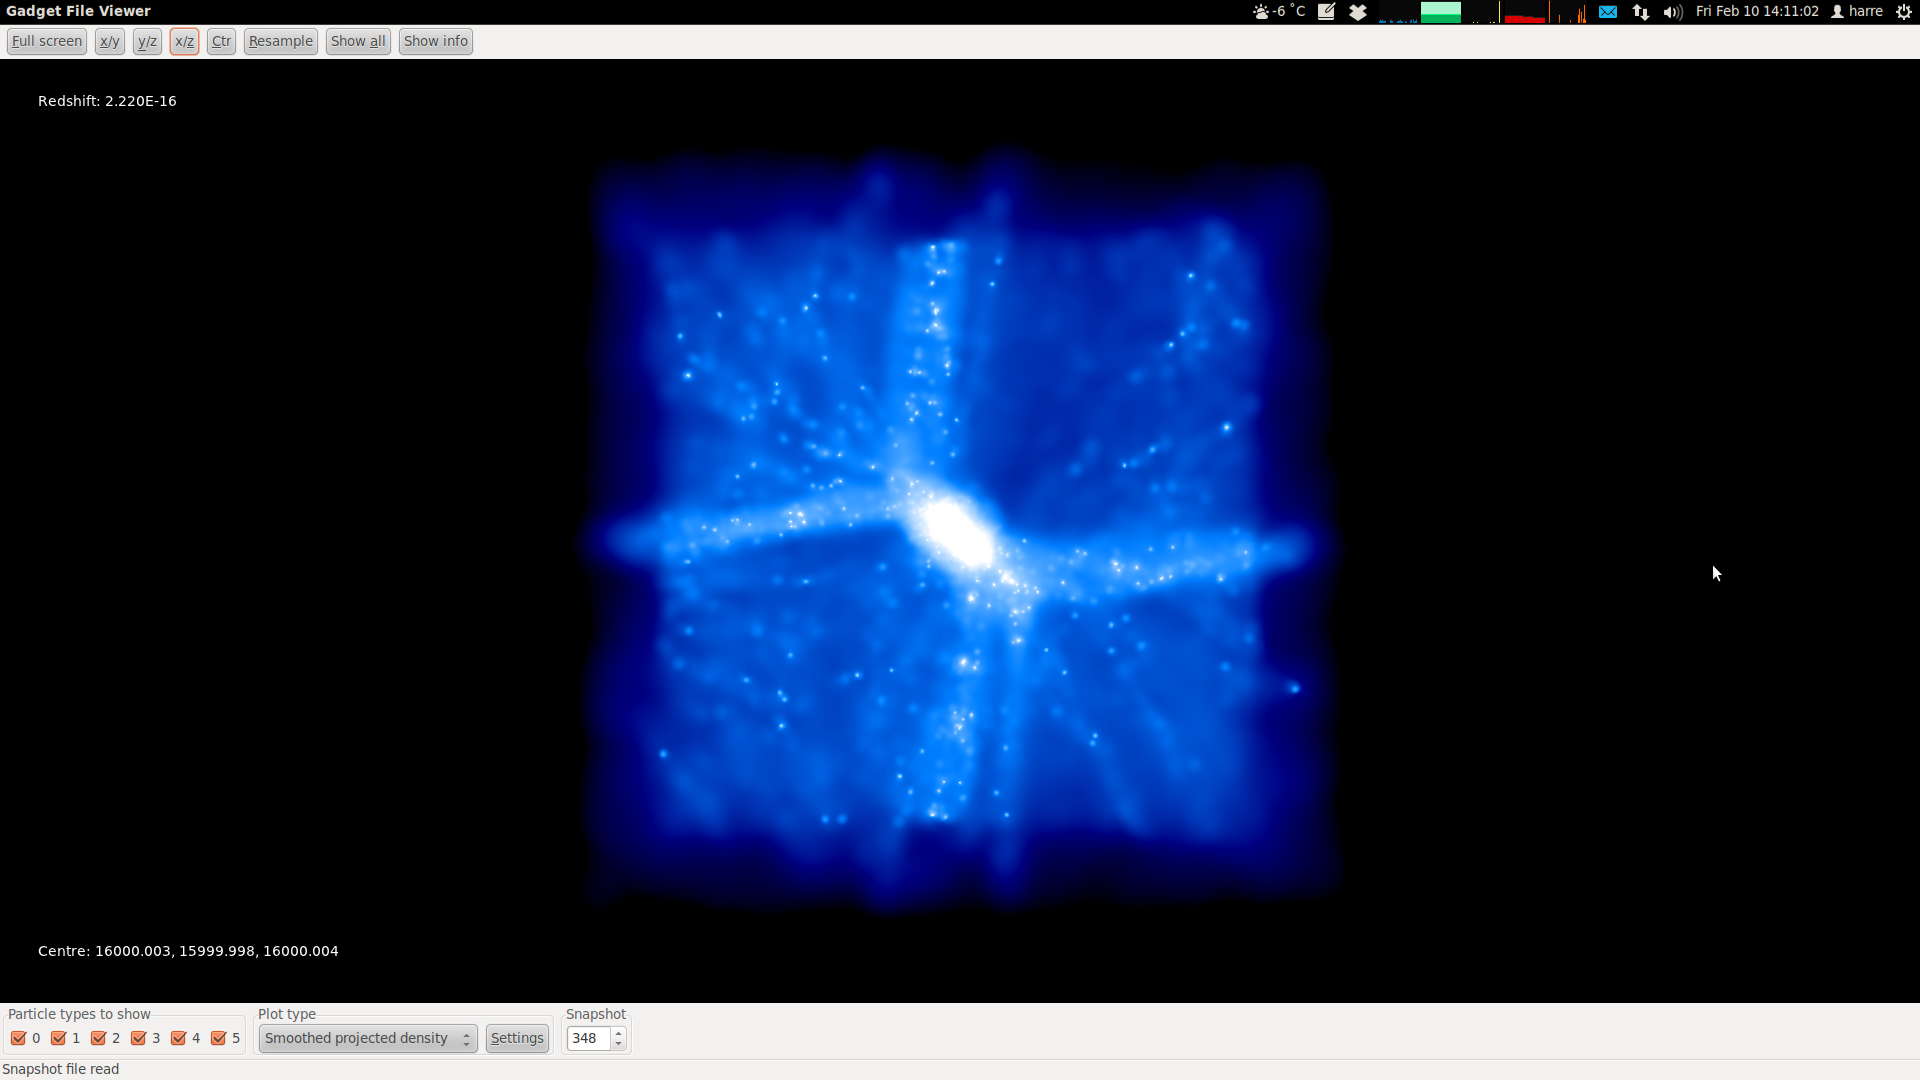
\includegraphics[scale=0.12]{drd5_r256_2/2.png} 

\textsc{rockstarred} $\surd$ (lasted about 9000minutes) \\
\textsc{consistenttreed} $\surd$ \\ 
is being galacticussed $\rightarrow$ job seems to run! \\
\begin{verbatim}
no: A fatal error occurred! Backtrace for this error:
#0  0x2B3F2E65E897
#1  0x2B3F2E65EE4E
#2  0x301763648F
#3  0x487AA0 in __merger_tree_read_MOD_build_descendent_pointers
#4  0x48ADC3 in __merger_tree_read_MOD_merger_tree_read_do
#5  0x48205E in __merger_tree_construction_MOD_merger_tree_create
#6  0x46F469 in __galacticus_tasks_evolve_tree_MOD_galacticus_task_evolve_tree._omp_fn.0 at galacticus.tasks.evolve_tree
.F90:0
#7  0x46F9C4 in __galacticus_tasks_evolve_tree_MOD_galacticus_task_evolve_tree
#8  0x46FA4F in __galacticus_tasks_MOD_galacticus_task_do
#9  0x4600E4 in MAIN__ at Galacticus.F90:0
\end{verbatim}
$\rightarrow$ re-converted with bugfixed converter (v0.3) \\
galacticus running on SGE \\
$\rightarrow$ gadgetviewer: simulation has "artificial" cross 
$\rightarrow$ DUMP IT ?


\newpage
\subsubsection{fuenfincr256\_1}

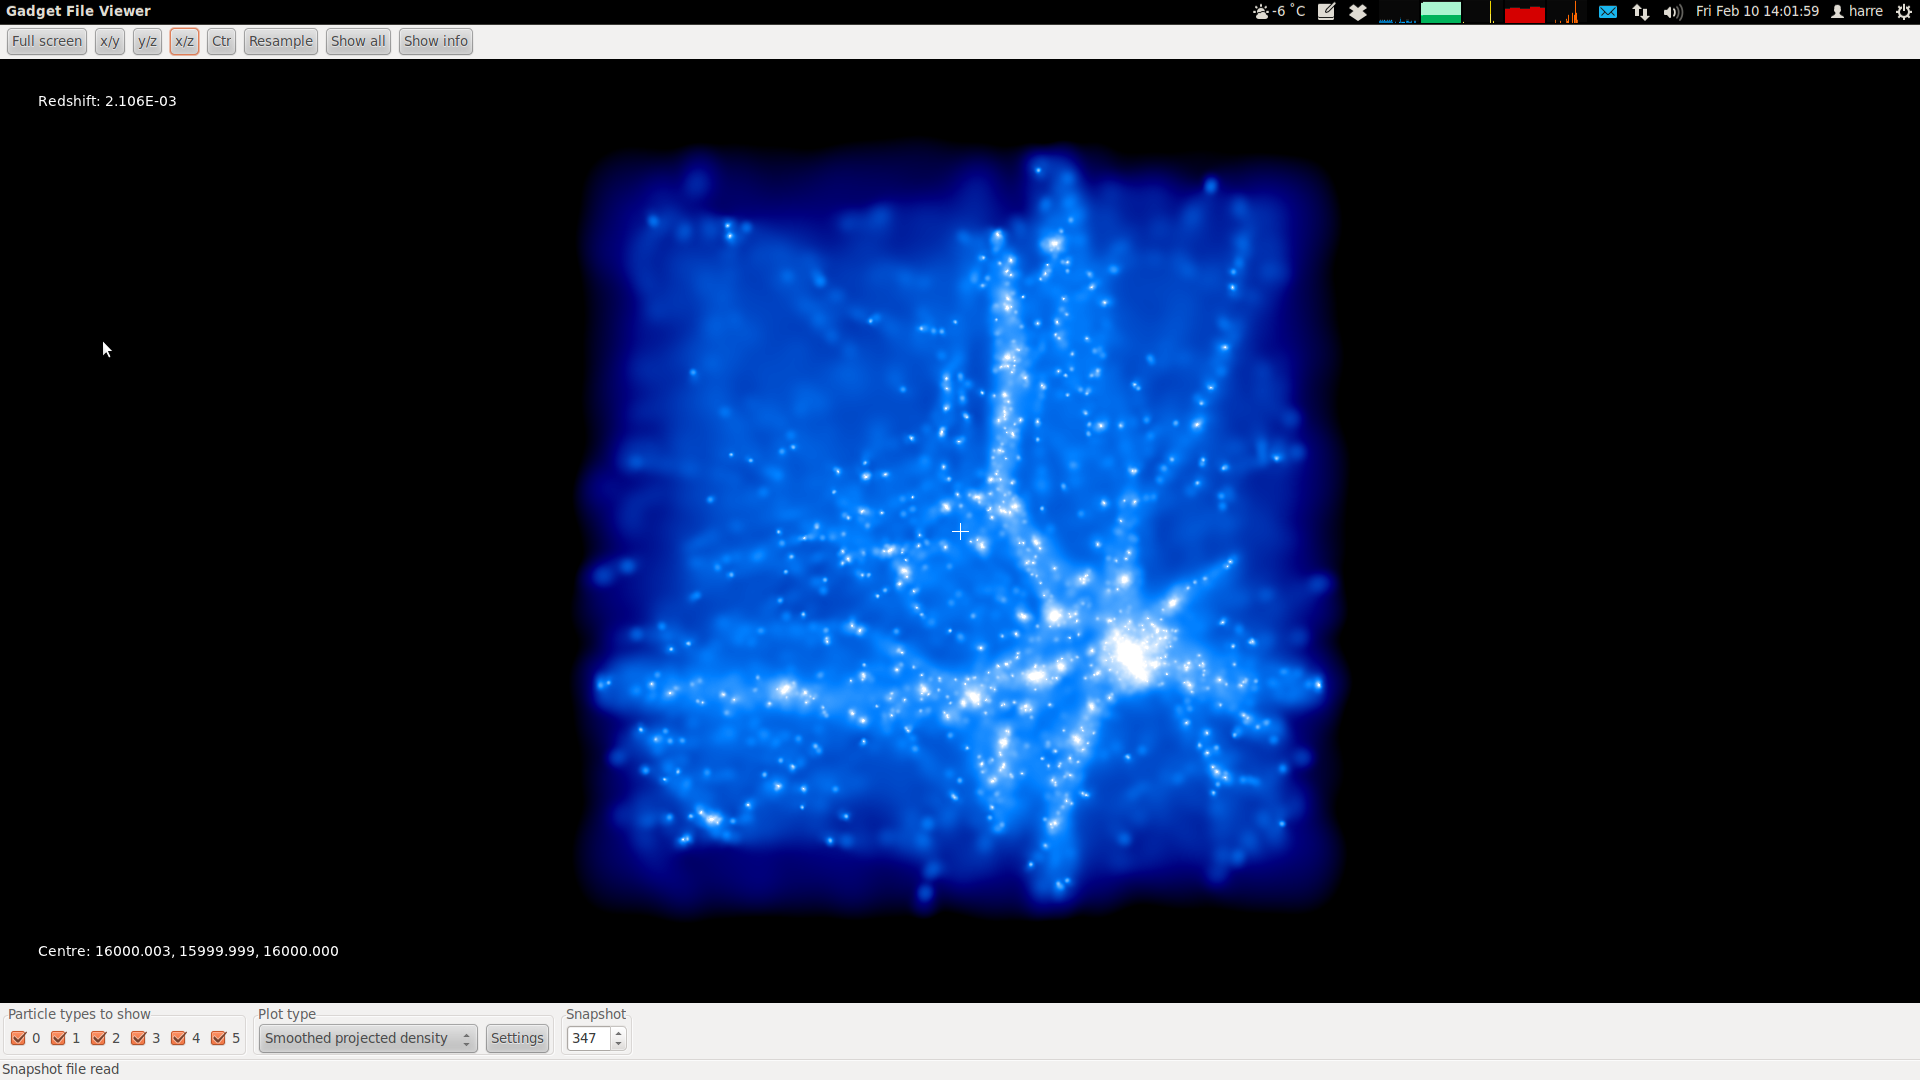
\includegraphics[scale=0.12]{fuenfincr256_1/1.png} 
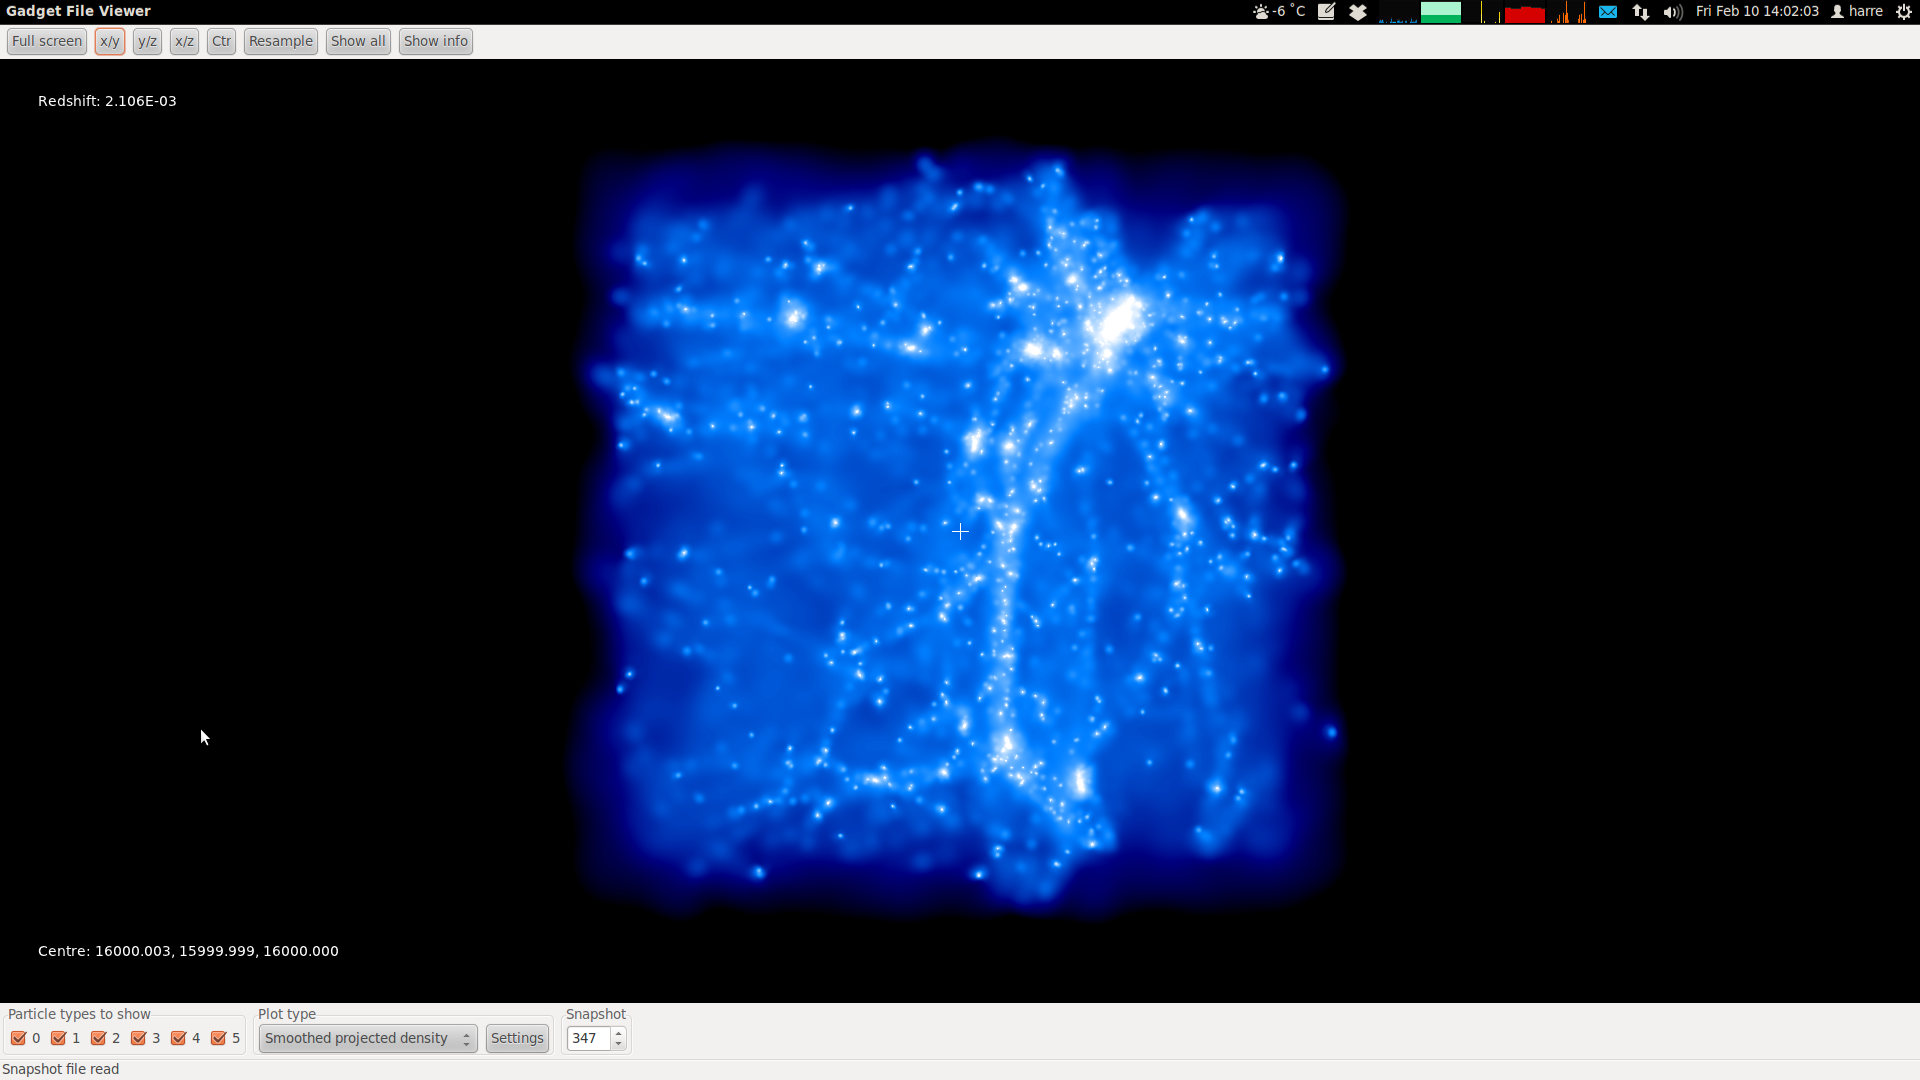
\includegraphics[scale=0.12]{fuenfincr256_1/2.png}

\textsc{rockstarred} $\surd$ \\ \textsc{consistenttreed} $\surd$
\\ \textsc{galacticus}: 
\begin{verbatim}
Fatal error in Build_Descendent_Pointers():
failed to find descendent node: 12048576 of 12014628
galacticus.sh: line 67:  5751 Aborted  
\end{verbatim}
tree copied to markus transfer \\
$\rightarrow$ re-converted with bugfixed converter \\
\begin{verbatim}
 Running model....... 
  Reading data for metallicity log10(Z/Z_Solar) = 0.198
   Found 188 ages in the file
  Found 1963 wavelengths in the file
gsl: ../../../../roots/brent.c:57: ERROR: function value is not finite
Default GSL error handler invoked.
\end{verbatim}
$\rightarrow$ E-Mail to Andrew \\

\newpage
\subsubsection{fuenfincr256\_2 $\rightarrow$ dump!}

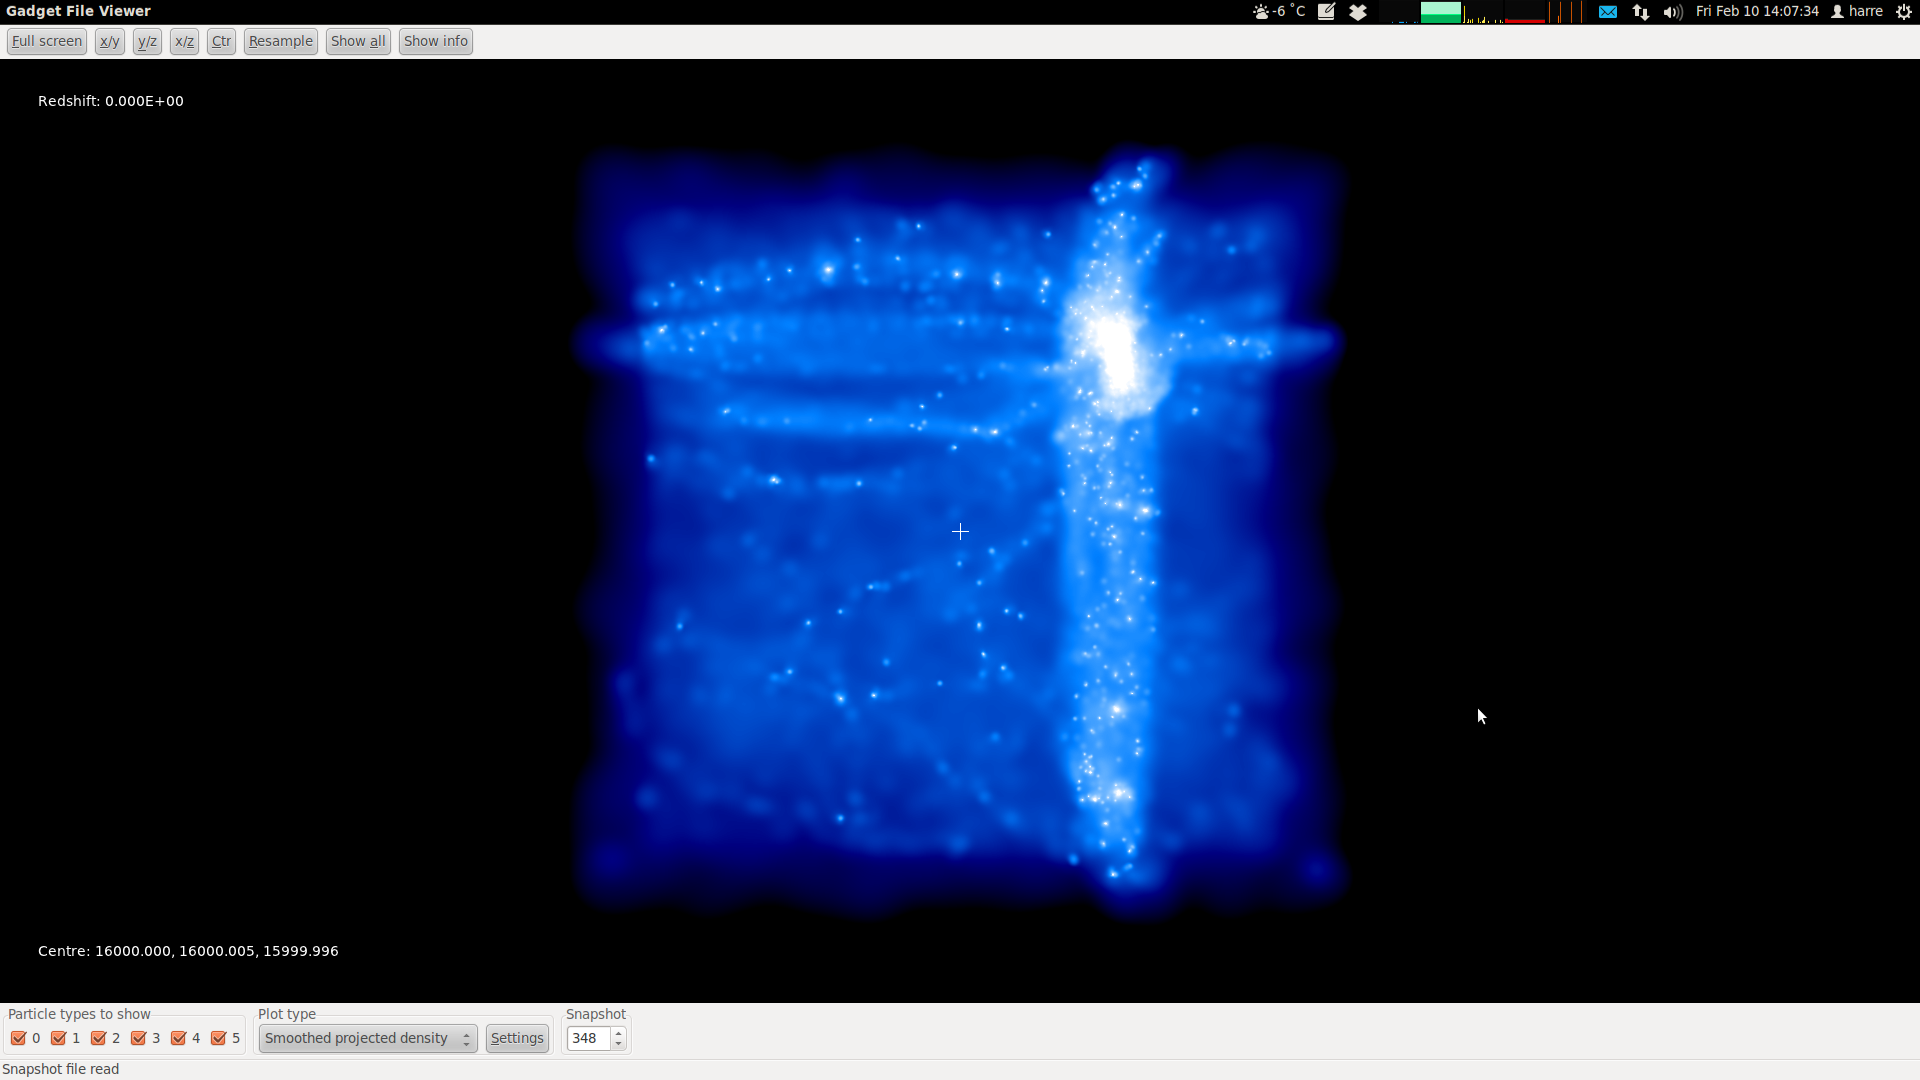
\includegraphics[scale=0.12]{fuenfincr256_2/1.png} 
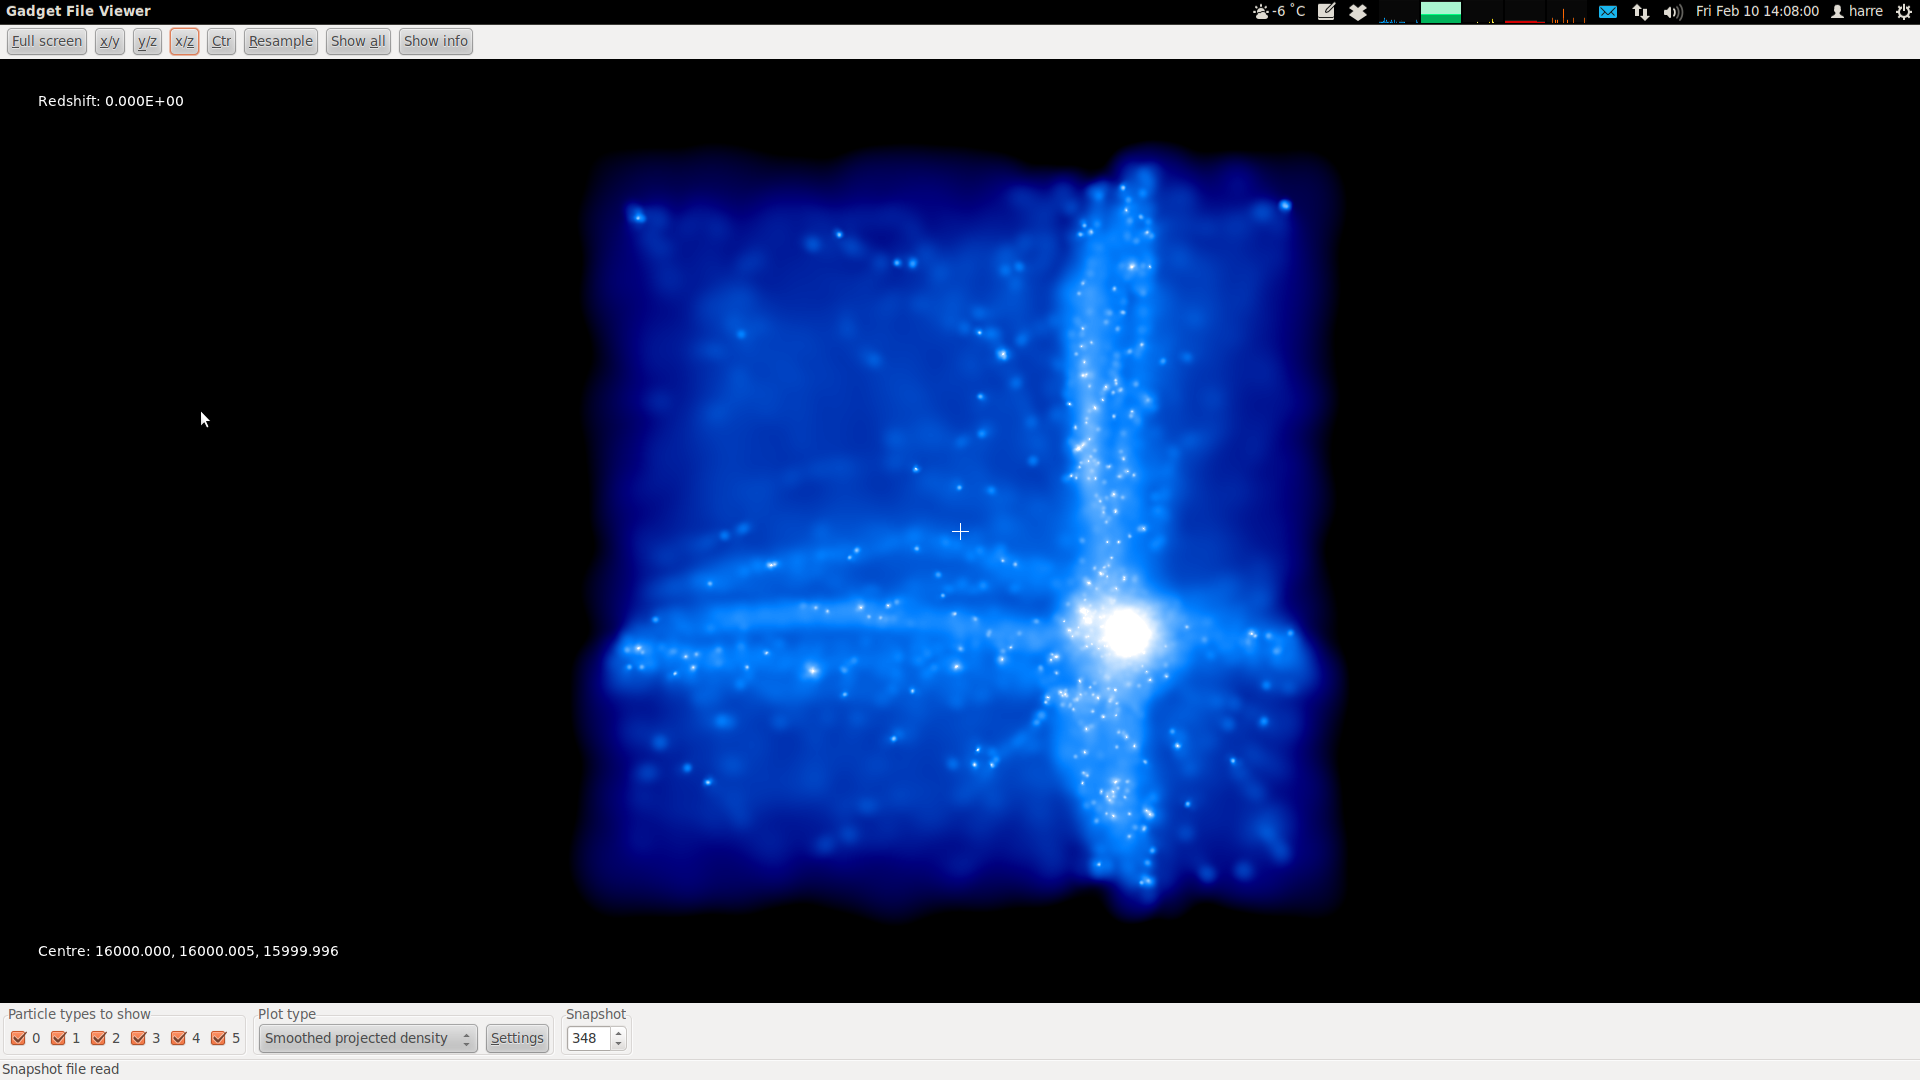
\includegraphics[scale=0.12]{fuenfincr256_2/2.png}

\textsc{rockstarred} $\surd$ (lasted about 9000minutes) \\
\textsc{consistenttreed} $\surd$ \\ 
is being galacticussed $\rightarrow$ job seems to run! \\
 \textsc{galacticus}:
 \begin{verbatim}
Fatal error in Build_Descendent_Pointers():
failed to find descendent node 
\end{verbatim}
$\rightarrow$ re-converted with bugfixed converter (v0.3) \\
galacticus running on SGE
$\rightarrow$ gadgetviewer: simulation has "artificial" cross on right upper corner $\rightarrow$ DUMP IT ?






%
%dreikluane1 
%consistentrees: Error: too few halos at scale factor 0.135721 to calculate consistency metric. - this is still z~6
%$\rightarrow$ has to be re-rockstarred! 
%is being rockstarred (astro11)
%was rockstarred $\rightarrow$ out_lists practically empty
%$\rightarrow$ changed lenght conversion from 0.001 to 1000 $\rightarrow$ pff
%
%dreikluane2 
%consistentrees: >> folder /home/harre/simulations/gadget-structure-formation/dreikluane2/output//rockstar does not exist, simulation was not yet rockstarred!
%is being rockstarred (astro12)
%$\rightarrow$ killed! 
%
%dreikluane3 
%consistentrees: >> folder /home/harre/simulations/gadget-structure-formation/dreikluane3/output//rockstar does not exist, simulation was not yet rockstarred! 
%is being rockstared (astro21)
%$\rightarrow$ killed!  
%
%dreikluane5 
%Error: too few halos at scale factor 0.306878 to calculate consistency metric.
%Please remove this and all earlier timesteps from the scale file and rerun. $\rightarrow$ re-rockstar! 
%is being rockstared (astro16)
%$\rightarrow$ rockstarred 
%
%drkl5dx1 
%is being rockstarred (astro23)  
%$\rightarrow$ Error: too few halos at scale factor 0.330498 to calculate consistency metric.
%
%dr5d5_r256 
%is being rockstarred 
%is being consistentreed $\rightarrow$ find_parents_and_cleanup: find_parents_and_cleanup.c:130: lookup_new_id: Assertion `new_id' failed.
%find_parents_and_cleanup: find_parents_and_cleanup.c:130: lookup_new_id: Assertion `new_id' failed.
%Tree creation failed while executing "./find_parents_and_cleanup dr5d5_r256.cfg".
%(See errors above).
%$\rightarrow$ rerockstar! 
%$\rightarrow$ is being rerockstarred on astro-x4600-03


\end{document}




